
\section[Παράλληλη Υλοποίηση του Αλγόριθμου σε Κάρτα Γραφικών (Cuda)]{Παράλληλη Υλοποίηση του Αλγόριθμου σε Κάρτα\\[-0.8em] Γραφικών (Cuda)}

Για την παραλληλοποιήση σε cuda απλά μετέτρεψα την παράλληλη συνάρτηση που κάνει τα περάσματα της εικόνας από των κώδικα openmp για παραλληλοποιήση σε επεξεργαστή, στον αντίστοιχο κώδικα cuda. Οπότε κατέληξα στο παρακάτω kernel function που τρέχει στην GPU.

\begin{minted}[breaklines, breaksymbolright={}, breaksymbolleft={}, bgcolor=paraiso-light]{c}
 __global__ void crimmins_pass_kernel(uint8_t *out, const uint8_t *in,
                  int width, int height, int dx, int dy, int is_light)
 {
     int x = blockIdx.x * blockDim.x + threadIdx.x + 1;
     int y = blockIdx.y * blockDim.y + threadIdx.y + 1;

     if (x >= width - 1 || y >= height - 1) return;

     uint8_t a = in[(y - dy) * width + (x - dx)];
     uint8_t b = in[y * width + x];
     uint8_t c = in[(y + dy) * width + (x + dx)];

     b = is_light ? light_pass_logic_dev(a, b, c) :
                    dark_pass_logic_dev(a, b, c);

     out[y * width + x] = b;
 }
\end{minted}

Όπως και με της προηγούμενές υλοποιήσεις της συνάρτησης τα ορίσματα παραμένουν ίδια. Αρχικά υπολογίζουμε τις συντεταγμένες x και y που θα πάρει το κάθε νήμα που θα τρέξει το kernel με βάση τα blockId και τα threadId τους και προσθέτουμε 1 έτσι ώστε να ξεκινήσουν από το (1, 1) της εικόνας και όχι από το (0, 0). Έπειτα, ελέγχουμε αν δεν ξεπερνάει τα όρια της εικόνας και κάνουμε τον υπολογισμό των pixel με τον ίδιο τρόπο. Πάλι η επιλογή των ζευγαριών που θα κάνει το κάθε πέρασμα και το αν θα κάνει διόρθωση των σκοτεινών ή φωτεινών pixel επιλέγεται παραμετροποιημένα από τα ορίσματα της συνάρτησης. Οι συναρτήσεις της λογικής διόρθωσης είναι οι ίδιες απλά έβαλα στο όρισμα των συναρτήσεων \verb|__device__| για να μπορώ να τις καλέσω από την GPU.

Για να καλέσω το kernel έχω την ακόλουθη συνάρτηση. Αρχικοποιεί τα events για την μέτρηση χρόνου, φτιάχνει τα δύο buffers που θα έχουν την εικόνα στην μνήμη του GPU και την αντιγράφει εκεί. Έπειτα, ορίζουμε το μέγεθος του grid και των block, δηλαδή πόσα block θα χρησιμοποιήσουμε με πόσα threads το καθένα. Επέλεξα να έχω blocks με 32x32 threads (1024 threads). Τα blocks που χρειαζόμαστε υπολογίζονται με βάση τις διαστάσεις της εικόνας.
Μετά, καλώ το kernel 8 φορές για τα 8 περάσματα τις εικόνας και επαναλαμβάνω για όσες επαναλήψεις έχω. Τέλος, μεταφέρω το αποτέλεσμα στον host, κάνω free τις μεταβλητές και μετράω τον χρόνο που χρειάστηκε.

\begin{minted}[breaklines, breaksymbolright={}, breaksymbolleft={}, bgcolor=paraiso-light]{c}
 float crimmings_speckle_removal_filter_cuda(uint8_t *h_image,
             uint32_t width, uint32_t height, uint8_t iterations)
 {
     size_t numPixels = (size_t)(width * height);
     size_t bufBytes = numPixels * sizeof(uint8_t);

     cudaEvent_t start, stop;
     cudaEventCreate(&start);
     cudaEventCreate(&stop);
     cudaEventRecord(start, 0);

     uint8_t *d_in = NULL;
     uint8_t *d_out = NULL;
     CHECK_CUDA(cudaMalloc((void **)&d_in, bufBytes));
     CHECK_CUDA(cudaMalloc((void **)&d_out, bufBytes));

     CHECK_CUDA(cudaMemcpy(d_in, h_image, bufBytes, cudaMemcpyHostToDevice));
     CHECK_CUDA(cudaMemcpy(d_out, h_image, bufBytes, cudaMemcpyDeviceToDevice));

     dim3 block = {32, 32, 1};
     dim3 grid = {
         (uint32_t)((width + block.x - 3) / block.x),
         (uint32_t)((height + block.y - 3) / block.y),
         1
     };
     for (int iter = 0; iter < iterations; iter++) {
         for (int p = 0; p < 8; p++) {
             int is_light = (passes[p].pass_logic_func == light_pass_logic);

             crimmins_pass_kernel<<<grid, block>>>(
             d_out, d_in, width, height, passes[p].dx, passes[p].dy, is_light);

             SWAP(d_out, d_in);
         }
     }
     CHECK_CUDA(cudaMemcpy(h_image, d_out, bufBytes, cudaMemcpyDeviceToHost));

     cudaEventRecord(stop, 0);
     cudaEventSynchronize(stop);
     float time = 0;
     cudaEventElapsedTime(&time, start, stop);

     cudaEventDestroy(start);
     cudaEventDestroy(stop);

     cudaFree(d_buf1);
     cudaFree(d_buf2);
     return time * 1e-3f; // convert to sec
 }
\end{minted}

\section{Πειραματικά αποτελέσματα CUDA}

\begin{table}[H]
\caption*{\large 1 Iteration}
    \centering
    \begin{subtable}[t]{0.48\textwidth}
        \centering
        \pgfplotstabletypeset[
        col sep=tab,
        header=true,
        columns={cuda,{mri512.raw/1 (serial)},{mri512.raw/1 (parallel)},{mri512.raw/1 (speedup)}},
        columns/{mri512.raw/1 (serial)}/.style={column name=Ts,fixed,precision=4},
        columns/{mri512.raw/1 (parallel)}/.style={column name=Tp,fixed,precision=4},
        columns/{mri512.raw/1 (speedup)}/.style={column name=Sp,fixed,precision=3},
        column type=c,
        every first column/.style={column type=|c},
        column type/.add={|}{|},
        every head row/.style={
            before row=\hline,
            after row=\hline
        },
        every row/.style={
            before row=\hline
        },
        every last row/.style={
            after row=\hline
        }
        ]{./data/cudaCom.csv}
        \caption{mri512.raw with 1 iteration}
    \end{subtable}%
    \hfill
    \begin{subtable}[t]{0.48\textwidth}
        \centering
        \pgfplotstabletypeset[
        col sep=tab,
        header=true,
        columns={cuda,{mountain1024.raw/1 (serial)},{mountain1024.raw/1 (parallel)},{mountain1024.raw/1 (speedup)}},
        columns/threads/.style={column name=CPUs},
        columns/{mountain1024.raw/1 (serial)}/.style={column name=Ts,fixed,precision=4},
        columns/{mountain1024.raw/1 (parallel)}/.style={column name=Tp,fixed,precision=4},
        columns/{mountain1024.raw/1 (speedup)}/.style={column name=Sp,fixed,precision=2},
        column type=c,
        every first column/.style={column type=|c},
        column type/.add={|}{|},
        every head row/.style={
            before row=\hline,
            after row=\hline
        },
        every row/.style={
            before row=\hline
        },
        every last row/.style={
            after row=\hline
        }
        ]{./data/cudaCom.csv}
        \caption{mountain1024.raw with 1 iteration}
    \end{subtable}

    \vspace{8pt}

    \begin{subtable}[t]{0.48\textwidth}
        \centering
        \pgfplotstabletypeset[
        col sep=tab,
        header=true,
        columns={cuda,{mountain4096.raw/1 (serial)},{mountain4096.raw/1 (parallel)},{mountain4096.raw/1 (speedup)}},
        columns/{mountain4096.raw/1 (serial)}/.style={column name=Ts,fixed,precision=4},
        columns/{mountain4096.raw/1 (parallel)}/.style={column name=Tp,fixed,precision=4},
        columns/{mountain4096.raw/1 (speedup)}/.style={column name=Sp,fixed,precision=2},
        column type=c,
        every first column/.style={column type=|c},
        column type/.add={|}{|},
        every head row/.style={
            before row=\hline,
            after row=\hline
        },
        every row/.style={
            before row=\hline
        },
        every last row/.style={
            after row=\hline
        }
        ]{./data/cudaCom.csv}
        \caption{mountain4096.raw with 1 iteration}
    \end{subtable}%
    \hfill
    \begin{subtable}[t]{0.48\textwidth}
        \centering
        \pgfplotstabletypeset[
        col sep=tab,
        header=true,
        columns={cuda,{mountain30000.raw/1 (serial)},{mountain30000.raw/1 (parallel)},{mountain30000.raw/1 (speedup)}},
        columns/{mountain30000.raw/1 (serial)}/.style={column name=Ts,fixed,precision=4},
        columns/{mountain30000.raw/1 (parallel)}/.style={column name=Tp,fixed,precision=4},
        columns/{mountain30000.raw/1 (speedup)}/.style={column name=Sp,fixed,precision=2},
        column type=c,
        every first column/.style={column type=|c},
        column type/.add={|}{|},
        every head row/.style={
            before row=\hline,
            after row=\hline
        },
        every row/.style={
            before row=\hline
        },
        every last row/.style={
            after row=\hline
        }
        ]{./data/cudaCom.csv}
        \caption{mountain30000.raw with 1 iteration}
    \end{subtable}
\end{table}

\begin{table}[H]
\caption*{\large 4 Iterations}
    \centering
    \begin{subtable}[t]{0.48\textwidth}
        \centering
        \pgfplotstabletypeset[
        col sep=tab,
        header=true,
        columns={cuda,{mri512.raw/4 (serial)},{mri512.raw/4 (parallel)},{mri512.raw/4 (speedup)}},
        columns/{mri512.raw/4 (serial)}/.style={column name=Ts,fixed,precision=4},
        columns/{mri512.raw/4 (parallel)}/.style={column name=Tp,fixed,precision=4},
        columns/{mri512.raw/4 (speedup)}/.style={column name=Sp,fixed,precision=2},
        column type=c,
        every first column/.style={column type=|c},
        column type/.add={|}{|},
        every head row/.style={
            before row=\hline,
            after row=\hline
        },
        every row/.style={
            before row=\hline
        },
        every last row/.style={
            after row=\hline
        }
        ]{./data/cudaCom.csv}
        \caption{mri512.raw with 4 iteration}
    \end{subtable}%
    \hfill
    \begin{subtable}[t]{0.48\textwidth}
        \centering
        \pgfplotstabletypeset[
        col sep=tab,
        header=true,
        columns={cuda,{mountain1024.raw/4 (serial)},{mountain1024.raw/4 (parallel)},{mountain1024.raw/4 (speedup)}},
        columns/threads/.style={column name=CPUs},
        columns/{mountain1024.raw/4 (serial)}/.style={column name=Ts,fixed,precision=4},
        columns/{mountain1024.raw/4 (parallel)}/.style={column name=Tp,fixed,precision=4},
        columns/{mountain1024.raw/4 (speedup)}/.style={column name=Sp,fixed,precision=2},
        column type=c,
        every first column/.style={column type=|c},
        column type/.add={|}{|},
        every head row/.style={
            before row=\hline,
            after row=\hline
        },
        every row/.style={
            before row=\hline
        },
        every last row/.style={
            after row=\hline
        }
        ]{./data/cudaCom.csv}
        \caption{mountain1024.raw with 4 iteration}
    \end{subtable}

    \vspace{8pt}

    \begin{subtable}[t]{0.48\textwidth}
        \centering
        \pgfplotstabletypeset[
        col sep=tab,
        header=true,
        columns={cuda,{mountain4096.raw/4 (serial)},{mountain4096.raw/4 (parallel)},{mountain4096.raw/4 (speedup)}},
        columns/{mountain4096.raw/4 (serial)}/.style={column name=Ts,fixed,precision=4},
        columns/{mountain4096.raw/4 (parallel)}/.style={column name=Tp,fixed,precision=4},
        columns/{mountain4096.raw/4 (speedup)}/.style={column name=Sp,fixed,precision=2},
        column type=c,
        every first column/.style={column type=|c},
        column type/.add={|}{|},
        every head row/.style={
            before row=\hline,
            after row=\hline
        },
        every row/.style={
            before row=\hline
        },
        every last row/.style={
            after row=\hline
        }
        ]{./data/cudaCom.csv}
        \caption{mountain4096.raw with 4 iteration}
    \end{subtable}%
    \hfill
    \begin{subtable}[t]{0.48\textwidth}
        \centering
        \pgfplotstabletypeset[
        col sep=tab,
        header=true,
        columns={cuda,{mountain30000.raw/4 (serial)},{mountain30000.raw/4 (parallel)},{mountain30000.raw/4 (speedup)}},
        columns/{mountain30000.raw/4 (serial)}/.style={column name=Ts,fixed,precision=4},
        columns/{mountain30000.raw/4 (parallel)}/.style={column name=Tp,fixed,precision=4},
        columns/{mountain30000.raw/4 (speedup)}/.style={column name=Sp,fixed,precision=2},
        column type=c,
        every first column/.style={column type=|c},
        column type/.add={|}{|},
        every head row/.style={
            before row=\hline,
            after row=\hline
        },
        every row/.style={
            before row=\hline
        },
        every last row/.style={
            after row=\hline
        }
        ]{./data/cudaCom.csv}
        \caption{mountain30000.raw with 4 iteration}
    \end{subtable}
\end{table}

\begin{table}[H]
\caption*{\large 10 Iterations}
    \centering
    \begin{subtable}[t]{0.48\textwidth}
        \centering
        \pgfplotstabletypeset[
        col sep=tab,
        header=true,
        columns={cuda,{mri512.raw/10 (serial)},{mri512.raw/10 (parallel)},{mri512.raw/10 (speedup)}},
        columns/{mri512.raw/10 (serial)}/.style={column name=Ts,fixed,precision=4},
        columns/{mri512.raw/10 (parallel)}/.style={column name=Tp,fixed,precision=4},
        columns/{mri512.raw/10 (speedup)}/.style={column name=Sp,fixed,precision=2},
        column type=c,
        every first column/.style={column type=|c},
        column type/.add={|}{|},
        every head row/.style={
            before row=\hline,
            after row=\hline
        },
        every row/.style={
            before row=\hline
        },
        every last row/.style={
            after row=\hline
        }
        ]{./data/cudaCom.csv}
        \caption{mri512.raw with 10 iteration}
    \end{subtable}%
    \hfill
    \begin{subtable}[t]{0.48\textwidth}
        \centering
        \pgfplotstabletypeset[
        col sep=tab,
        header=true,
        columns={cuda,{mountain1024.raw/10 (serial)},{mountain1024.raw/10 (parallel)},{mountain1024.raw/10 (speedup)}},
        columns/threads/.style={column name=CPUs},
        columns/{mountain1024.raw/10 (serial)}/.style={column name=Ts,fixed,precision=4},
        columns/{mountain1024.raw/10 (parallel)}/.style={column name=Tp,fixed,precision=4},
        columns/{mountain1024.raw/10 (speedup)}/.style={column name=Sp,fixed,precision=2},
        column type=c,
        every first column/.style={column type=|c},
        column type/.add={|}{|},
        every head row/.style={
            before row=\hline,
            after row=\hline
        },
        every row/.style={
            before row=\hline
        },
        every last row/.style={
            after row=\hline
        }
        ]{./data/cudaCom.csv}
        \caption{mountain1024.raw with 10 iteration}
    \end{subtable}

    \vspace{8pt}

    \begin{subtable}[t]{0.48\textwidth}
        \centering
        \pgfplotstabletypeset[
        col sep=tab,
        header=true,
        columns={cuda,{mountain4096.raw/10 (serial)},{mountain4096.raw/10 (parallel)},{mountain4096.raw/10 (speedup)}},
        columns/{mountain4096.raw/10 (serial)}/.style={column name=Ts,fixed,precision=4},
        columns/{mountain4096.raw/10 (parallel)}/.style={column name=Tp,fixed,precision=4},
        columns/{mountain4096.raw/10 (speedup)}/.style={column name=Sp,fixed,precision=2},
        column type=c,
        every first column/.style={column type=|c},
        column type/.add={|}{|},
        every head row/.style={
            before row=\hline,
            after row=\hline
        },
        every row/.style={
            before row=\hline
        },
        every last row/.style={
            after row=\hline
        }
        ]{./data/cudaCom.csv}
        \caption{mountain4096.raw with 10 iteration}
    \end{subtable}%
    \hfill
    \begin{subtable}[t]{0.48\textwidth}
        \centering
        \pgfplotstabletypeset[
        col sep=tab,
        header=true,
        columns={cuda,{mountain30000.raw/10 (serial)},{mountain30000.raw/10 (parallel)},{mountain30000.raw/10 (speedup)}},
        columns/{mountain30000.raw/10 (serial)}/.style={column name=Ts,fixed,precision=4},
        columns/{mountain30000.raw/10 (parallel)}/.style={column name=Tp,fixed,precision=4},
        columns/{mountain30000.raw/10 (speedup)}/.style={column name=Sp,fixed,precision=2},
        column type=c,
        every first column/.style={column type=|c},
        column type/.add={|}{|},
        every head row/.style={
            before row=\hline,
            after row=\hline
        },
        every row/.style={
            before row=\hline
        },
        every last row/.style={
            after row=\hline
        }
        ]{./data/cudaCom.csv}
        \caption{mountain30000.raw with 10 iteration}
    \end{subtable}
\end{table}

Παρατηρούμε, ότι για μικρές εικόνες (μικρού μεγέθους πρόβλημα) ο χρόνος που χρειάζεται για να τρέξει στην GPU είναι μεγαλύτερος από τον σειριακό. Αυτό συμβαίνει γιατί ο χρόνος που χρειάζεται για να μεταφέρει τα δεδομένα των εικόνων από την RAM στην VRAM είναι μεγαλύτερος από ότι να τρέξει ο αλγόριθμος σειριακά. Για μεγαλύτερες εικόνες βλέπουμε να αυξάνει η επιτάχυνση κατά πολύ. Σημαντικό, εδώ είναι να πούμε ότι οι χρόνοι που χρειάζεται για να τρέξει ο αλγόριθμος στην GPU παραμένει σχετικά σταθερός γιατί το ένα πέρασμα της εικόνας γίνεται παράλληλα για όλα τα pixel όσο η εικόνα μπορεί να χωρέσει ολόκληρη στα threads της GPU.

\section{Σύγκριση των υλοποιήσεων}

\begin{figure}[H]
    \centering
    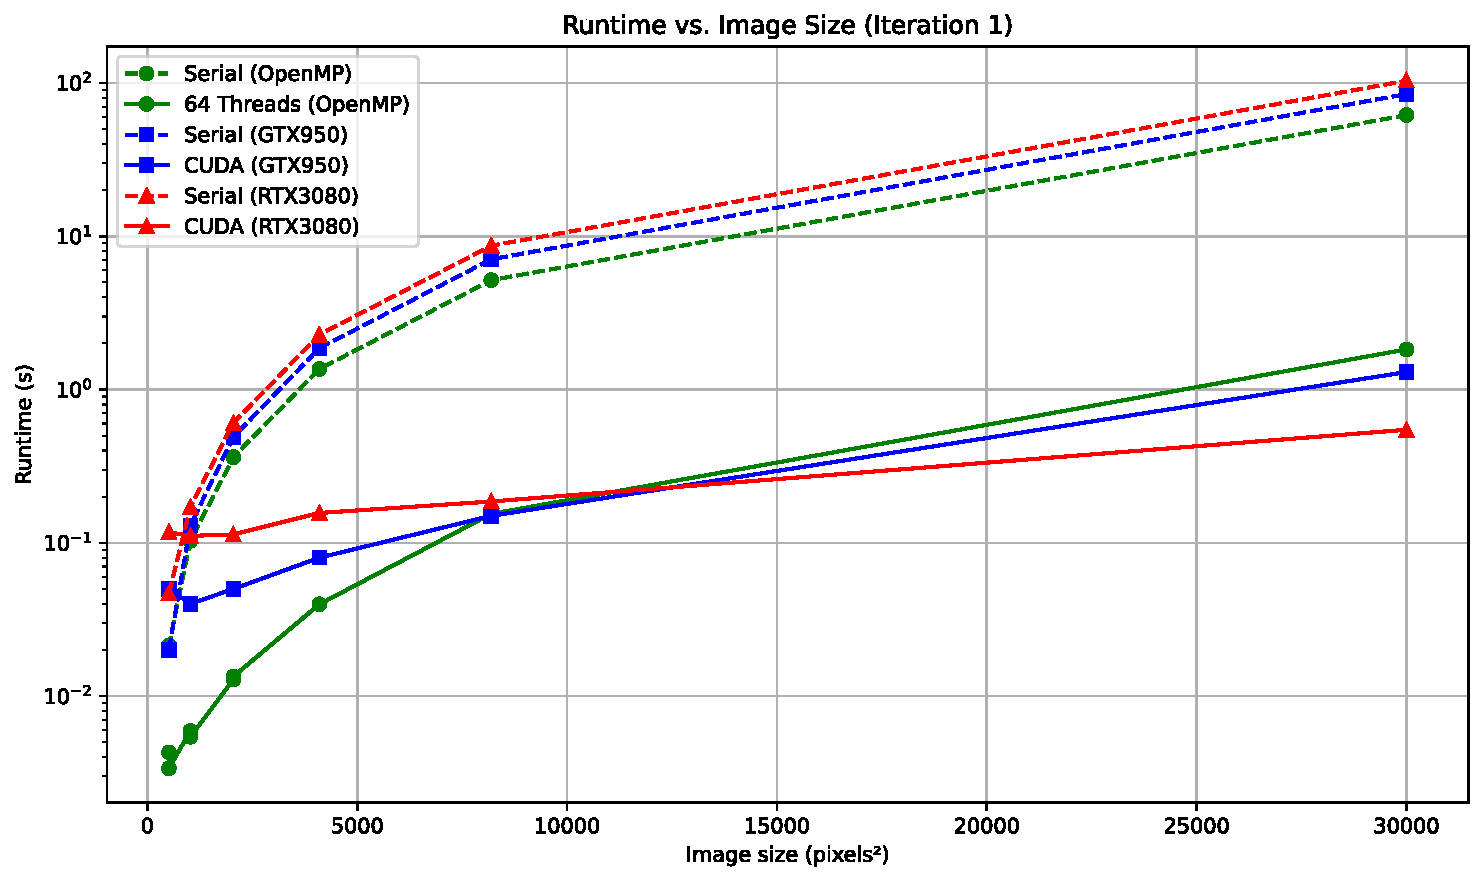
\includegraphics[width=\linewidth]{./pics/runtimeCurves_1.pdf}
    \caption{Χρόνος εκτέλεσης αλγορίθμου προς μέγεθος προβλήματος για μία επανάληψη}
\end{figure}

\begin{figure}[H]
    \centering
    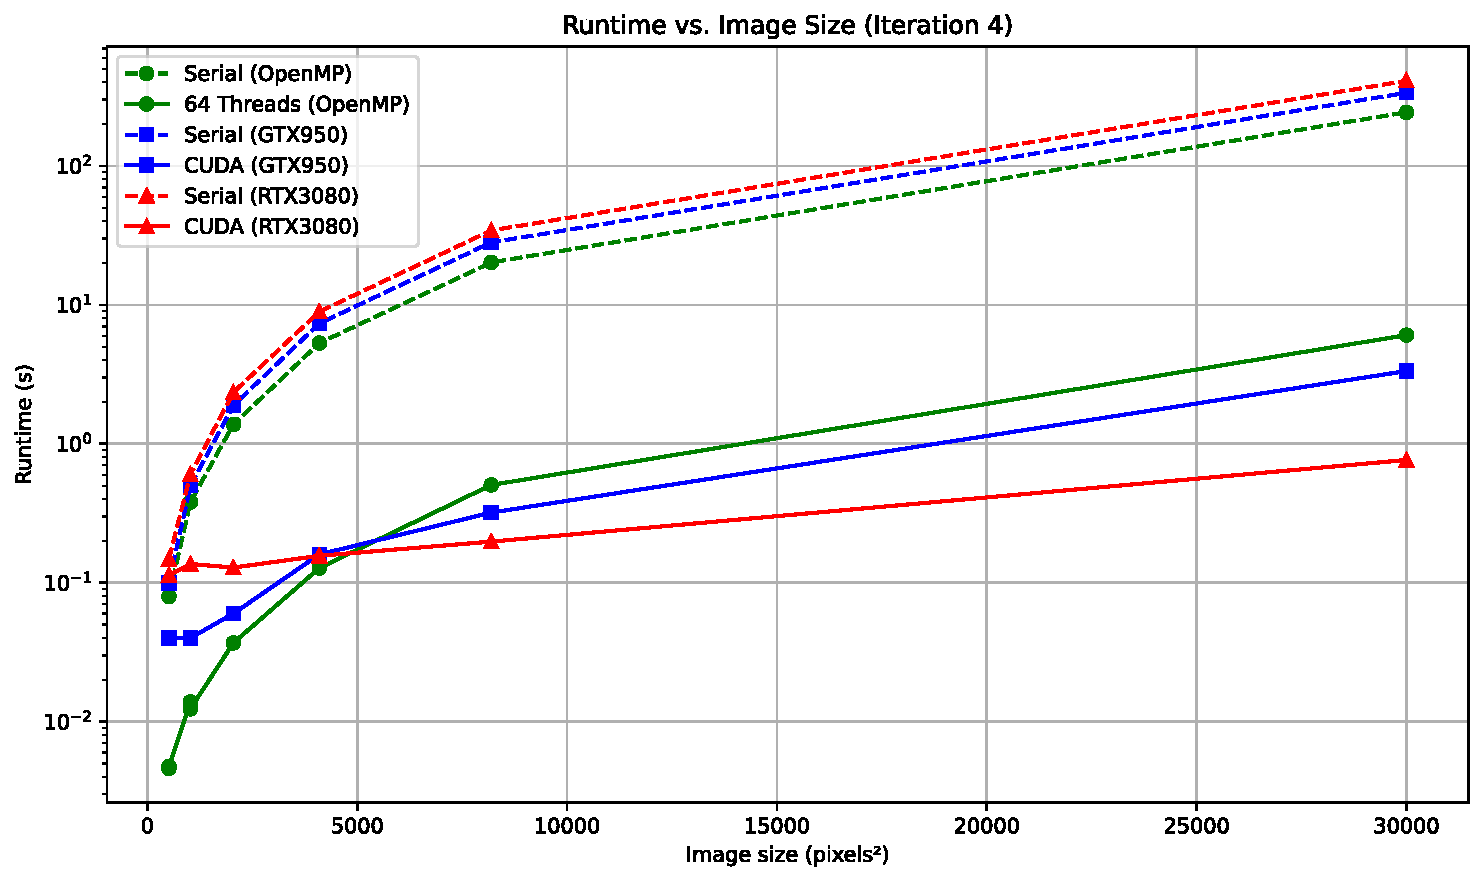
\includegraphics[width=\linewidth]{./pics/runtimeCurves_4.pdf}
    \caption{Χρόνος εκτέλεσης αλγορίθμου προς μέγεθος προβλήματος για τέσσερις επανάληψη}
\end{figure}

\begin{figure}[H]
    \centering
    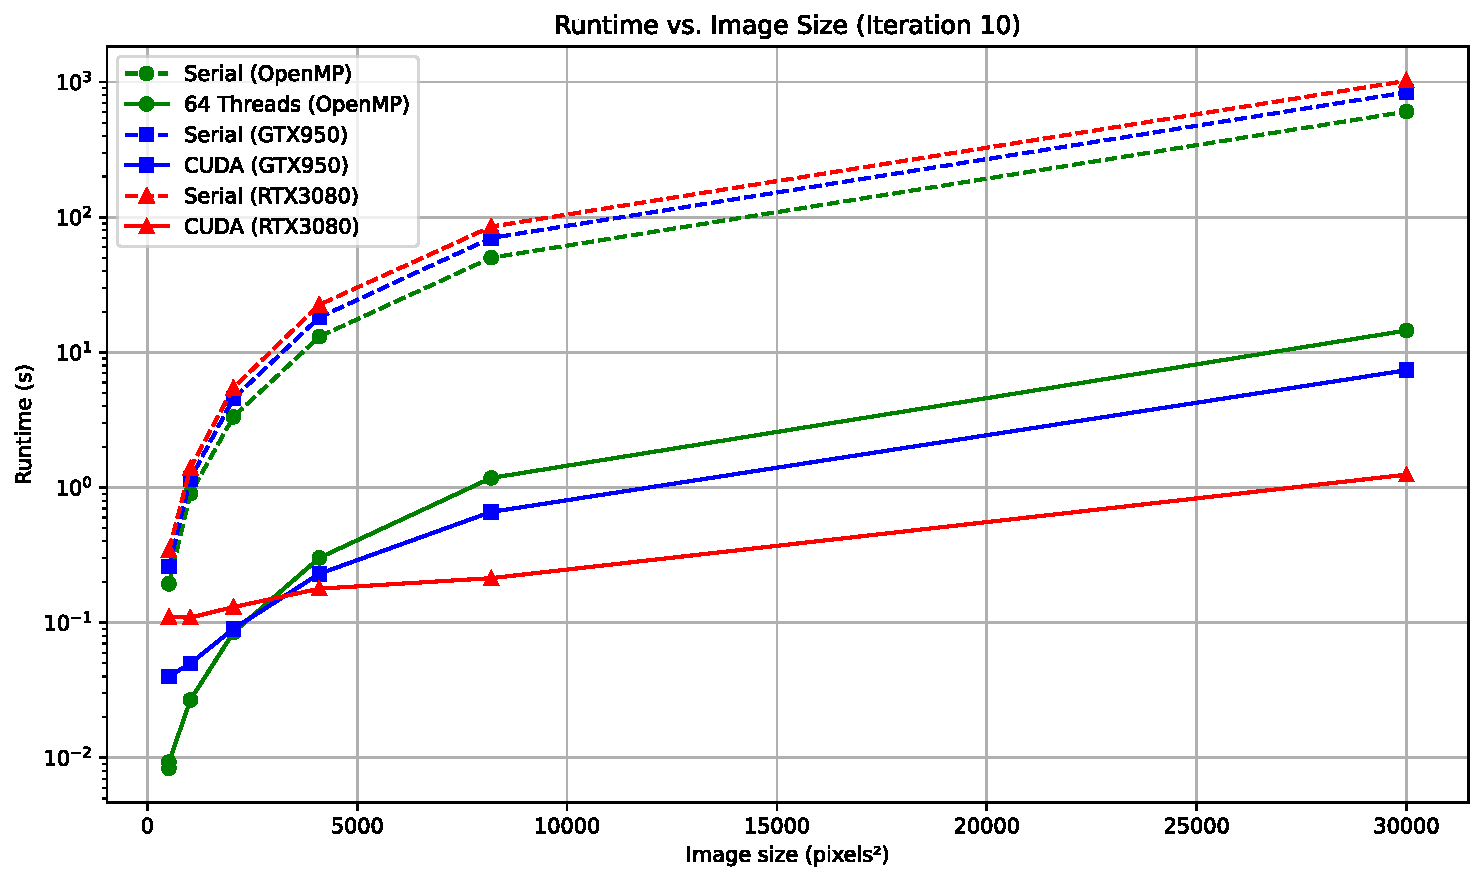
\includegraphics[width=\linewidth]{./pics/runtimeCurves_10.pdf}
    \caption{Χρόνος εκτέλεσης αλγορίθμου προς μέγεθος προβλήματος για δέκα επανάληψη}
\end{figure}

Αρχικά, βλέπουμε ότι οι χρόνοι του σειριακού αλγόριθμου αυξάνεται εκθετικά όσο αυξάνεται το μέγεθος της εικόνας. Ο χρόνος των παράλληλων αλγορίθμων στην GPU παραμένουν σχετικά σταθεροί.

\begin{figure}[H]
    \centering
    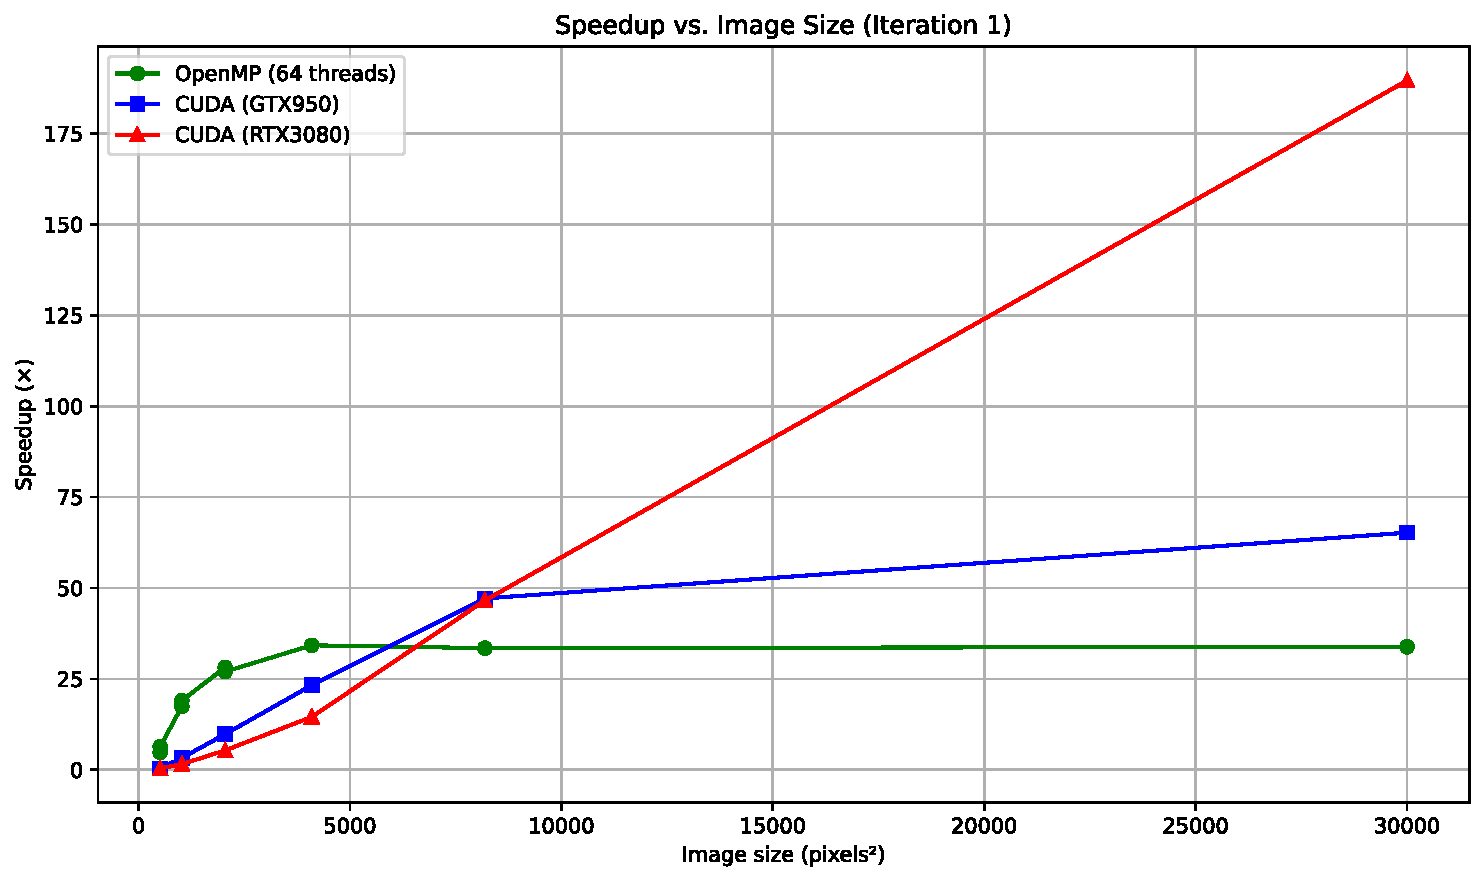
\includegraphics[width=\linewidth]{./pics/speedupCurves_1.pdf}
    \caption{Επιτάχυνση του αλγορίθμου προς το μέγεθος του προβλήματος για μία επανάληψη}
\end{figure}

\begin{figure}[H]
    \centering
    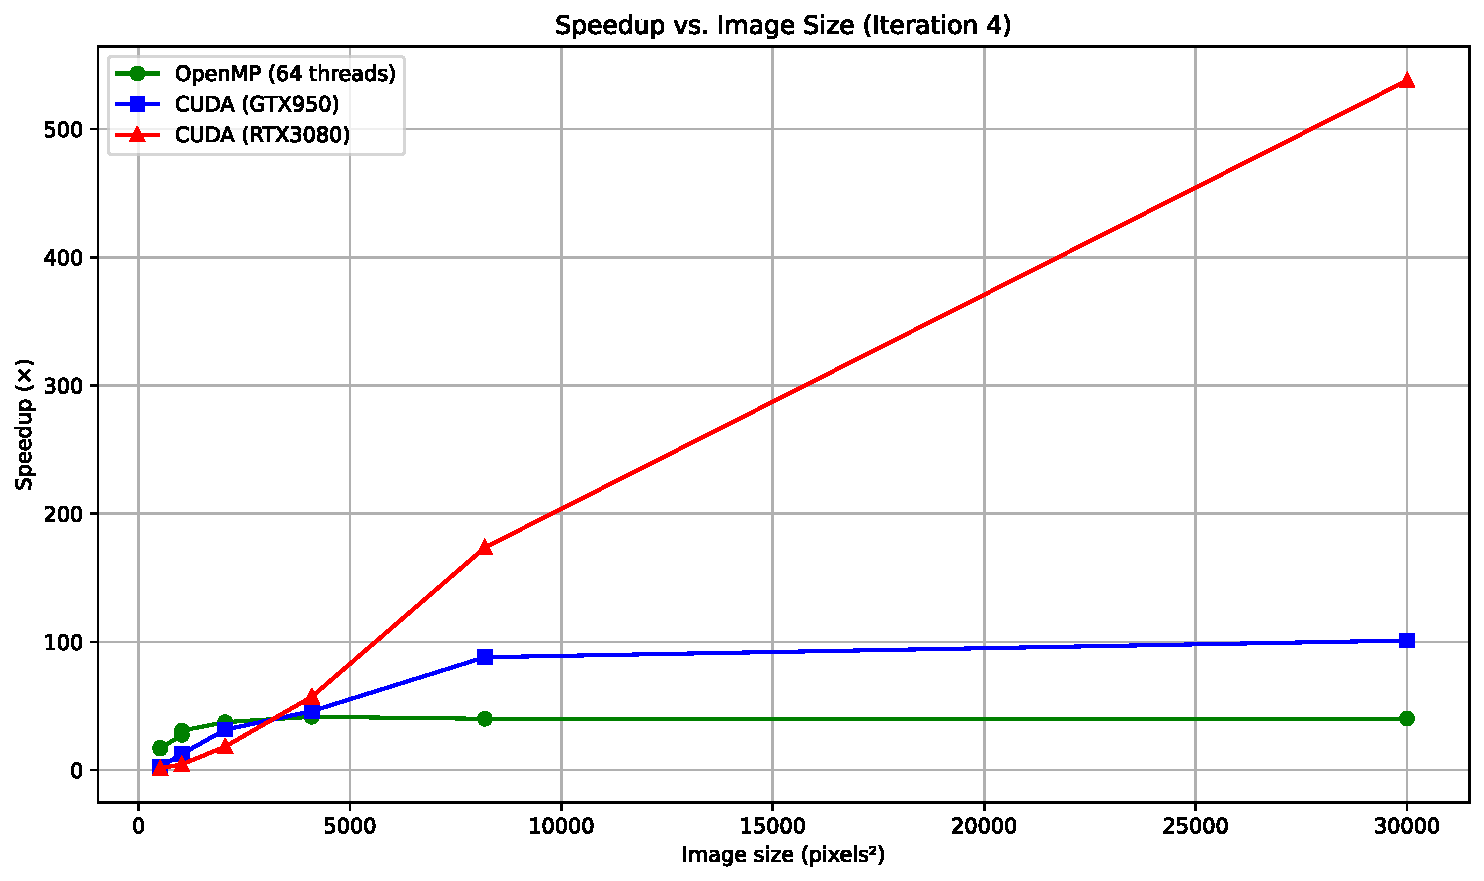
\includegraphics[width=\linewidth]{./pics/speedupCurves_4.pdf}
    \caption{Επιτάχυνση του αλγορίθμου προς το μέγεθος του προβλήματος για τέσσερις επαναλήψεις}
\end{figure}

\begin{figure}[H]
    \centering
    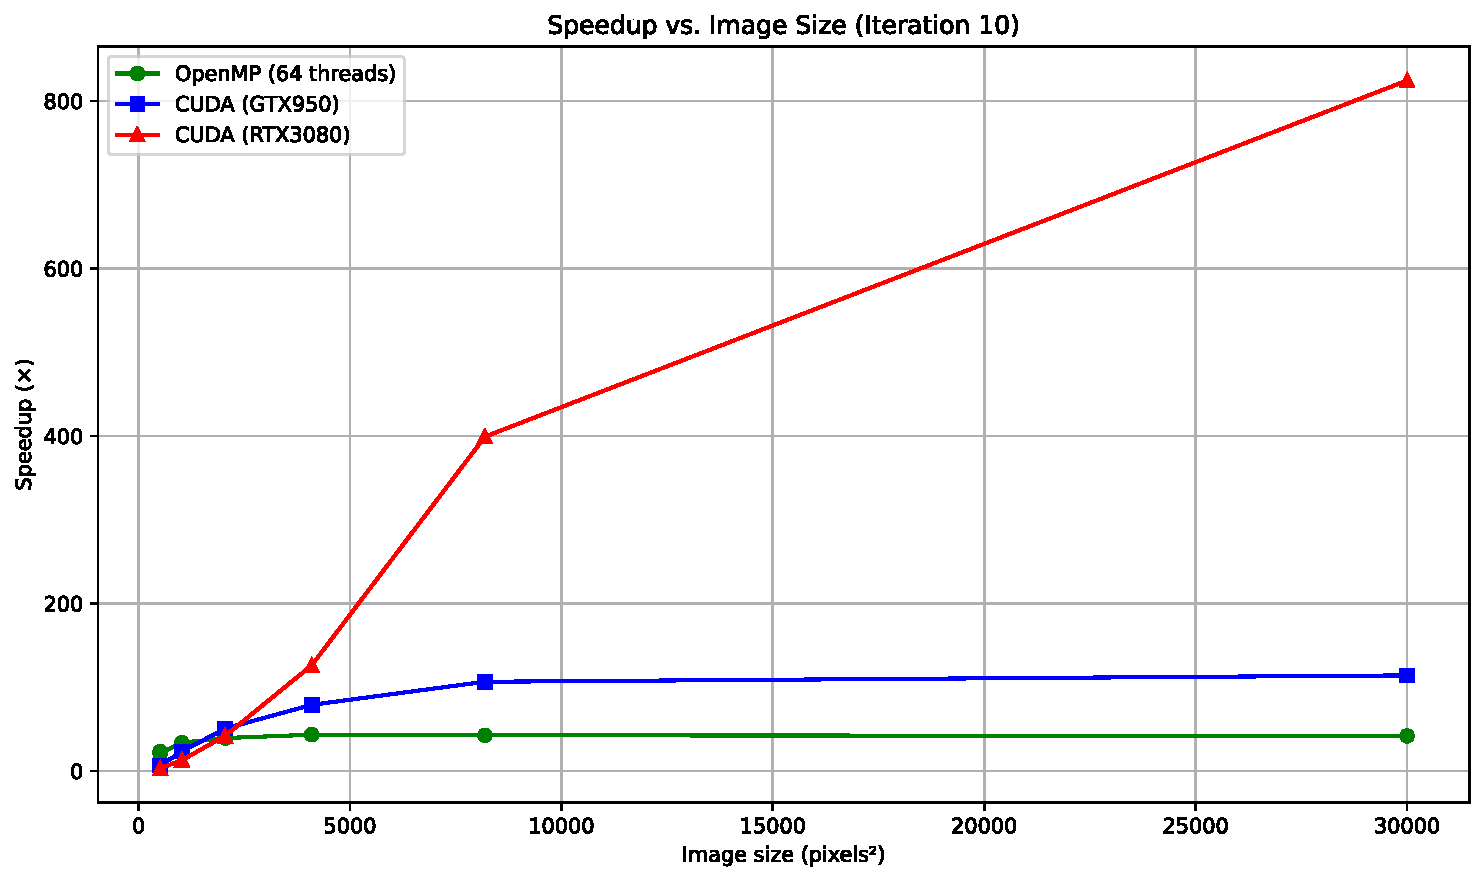
\includegraphics[width=\linewidth]{./pics/speedupCurves_10.pdf}
    \caption{Επιτάχυνση του αλγορίθμου προς το μέγεθος του προβλήματος για δέκα επαναλήψεις}
\end{figure}

Για τον παράλληλο αλγόριθμο στην rtx3080 το speedup συνεχίζει να αυξάνεται γραμμικά οπότε δεν βλέπουμε εδώ τα όρια της πλατφόρμας, όπως βλέπουμε με την gtx950 ή τον 64 πυρήνων CPU.
